%!TEX root = ../thesis.tex
%*******************************************************************************
%****************************** Second Chapter *********************************
%*******************************************************************************

\chapter{Results of Physical Properties Calculations in Novel 2D Materials \label{chap:4}}

\ifpdf
    \graphicspath{{Chapter4/Figs/Raster/}{Chapter4/Figs/PDF/}{Chapter4/Figs/Vector/}}
\else
    \graphicspath{{Chapter4/Figs/Vector/}{Chapter4/Figs/}}
\fi


\nocite{Yimamu2012}


In this and the next chapter, the main results of the thesis will be presented. In the \autoref{chap:1}, I have reviewed some of the early post-graphene 2D materials, and their physical properties in \autoref{chap:3}. As it has been defined, the properties discussed before belong to the basic property category. In this chapter, I will present my works on the determination of some of the advanced properties, namely thermal properties, piezoelectric properties, carrier mobility, magnetic properties and Li battery related properties. In addition, along with these new properties I will also introduce several new 2D materials on which the property determinations were carried out. They are phosphorene, monolayer Titanium trisulfide, penta-hexa-graphene and MXenes. Each of the sections below comes from one publication. 

\section[Thermal properties of phosphorene]{Thermal properties of phosphorene \footcite[This work is published in:][]{Aierken2015.thermalP} }


\subsection{Phosphorene}

Black phosphorene (black P) is a single atomic layer of layered material black phosphorus and has been successfully exfoliated \cite{Liu2014a,Li2014a}. Similar to the multiphase structures in phosphorus, there have been at least six different possible stable two dimensional allotropes of phosphorene were proposed\cite{Zhu2014,Guan2014a,Wu2015}. This multi-phase nature is because that in contrast to the C atoms of graphene, the P atoms in phosphorene have $sp^3$-hybridized orbitals. This is mainly caused by the extra valence electron of P atom in comparison to carbon. Indeed, if this extra electron is placed in a $sp^2$-hybridized structure, they would occupy the energetically unfavourable (antibonding) $\pi^*$ band. However, with $sp^3$-hybridization, a $\sigma$-bond network can be formed with three $sp^3$ orbitals and the other $sp^3$ orbital is used to host the remaining electron pair. This leads to an essentially tetragonal coordination of the P atoms and results in a buckled nature of $sp^3$-hybridized sheets, see \autoref{fig:phos_struc} for the structures. The out-of-plane positions of the atoms in $sp^3$-hybridized sheets give rise to various possible structural phases which are absent in $sp^2$-hybridized systems. Among those, black P, also referred as the $\alpha$ phase, is the most stable allotrope. However, the cohesive energy of blue phosphorene (blue P), or the $\beta$ phase, is only a few meV higher than that of black P, while other crystal structures are much less favourable with energy at least by $\sim$ 80 meV/atom higher.  

\begin{figure}[htbp] 
\centering
\includegraphics[width=0.8\linewidth]{phos_struc.eps}%
\caption[Black and blue phosphorene structures]{(a) and (b) are the one hexagonal rings of black P and blue P, their top viewed structures are shown in (c) and (d), respectively. Atoms are coloured in accordance with the names of the structures. Lighter coloured atoms mean they are lower in vertical position. Black boxes in top views are the primitive unit cell used in our calculations. }
\label{fig:phos_struc}
\end{figure}

Triggered by its realization, various physical properties of phosphorene have been explored. Electronically, black P is a semiconductor with a direct band gap at the $\Gamma$ point\cite{Zhu2014,dcakir}. Experimentally, photoluminescence excitation spectroscopy measured a quasi-particle band gap of 2.2 eV\cite{bp-ex-3}, which is larger than its bulk band gap, i.e. 0.31-0.33 eV\cite{Maruyama198199,Narita1983422}. Due to its electronic structure, black P has been proposed as a potential novel material in nanoelectronics and optoelectronics, especially in the infrared regime. High performance black P based transistors with a mobility up to 1000 cm$^2$/V$\cdot$s and an on/off ratio up to 10$^4$ at room temperature have been reported\cite{Li2014a,Liu2014a}. Similar to black P, blue P was predicted to be a semiconductor material with an indirect band gap around 2.00 eV\cite{Zhu2014}. Therefore, it can be potentially use for field-effect transistor applications. The high mobility and tunable finite band gap of phosphorene, among other promising properties\cite{Jain2015,Wei2014,Kou2014,Tahir2015,zhou2014}, make it an interesting new member of the 2D materials. Despite the mentioned studies that aimed to explore the physical properties of phosphorene, a more comprehensive knowledge of finite temperature effects on their properties haven't been reported. Given the fact that this knowledge could contribute to the acceleration in the progress towards its proposed applications, this study\cite{Aierken2015.thermalP} is urgently needed. To this end, here we explore the thermal properties of black p and blue p, their temperature-dependent lattice constant, thermal expansion coefficients, free energy and specific heat.

\subsection{Thermal expansion and Quasi-harmonic approximation}

\begin{figure}[htbp!] 
\centering
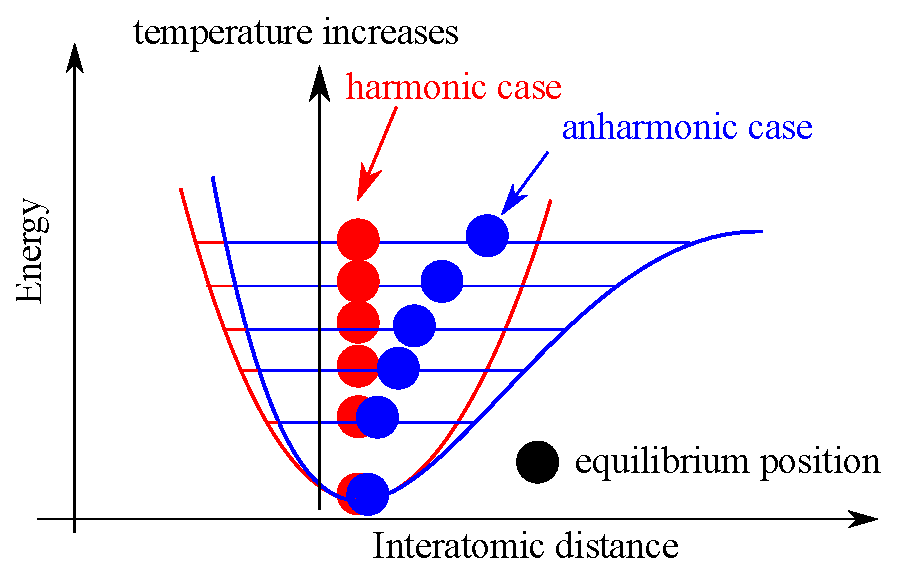
\includegraphics[width=0.8\linewidth]{anh_exp.eps}%
\caption{Schematic illustration of the relation between asymmetric interatomic potential and thermal expansion. }
\label{fig:anh_exp}
\end{figure}

The thermal expansion is the expansion of material's volume at finite temperature. As shown in \autoref{fig:anh_exp}, it is directly related to the asymmetric of interatomic potential where the equilibrium position shift towards the flatter side of the potential energy profile and stay far away from the steeper side as the temperature increases. In below we will see how we can include this anharmonic potential using an approximation. The thermal expansion coefficient $\alpha(T)$ are defined through the following formula: 
\begin{equation}
\alpha(T)=\frac{1}{a_0(T)}\frac{da_0(T)}{dT},
\end{equation}
where $T$ is the temperature, $a_0(T)$ is the equilibrium lattice parameter corresponding to the minimum of the Helmholtz free energy.

In order to describe the thermal expansion within DFT, one needs to go beyond the harmonic approximation that is used to calculate the phonon frequency as we discussed in \autoref{chap:3}. Harmonic approximation gives infinite thermal conductivity, infinite phonon lifetimes and temperature-independent vibrational and elastic properties, which are contradicted to experiment. Quasi-harmonic approximation (QHA)\cite{QHA1,QHA2,QHA3,Baroni39} is a way to include the approximated anharmonic effect through volume-dependent frequency within non-interacting phonons approximation. Although it is an implicitly inclusion of anharmonic effect, its dominant role in the thermal properties, that is two orders of magnitude larger than explicit anharmonic effect, make sure it can correctly describe the thermal properties up to melting point. Beyond this temperature, anharmonic effect will become important. QHA has been applied to a various compounds from semiconductors to metals and to Earth materials under extreme conditions\cite{Hamdi2006,Mounet2005,Grabowski2009,Karki2000} . In \autoref{fig:qha_gra}, the applications of QHA for graphite and graphene are shown. The agreement between experiment and QHA is good in a wide range of temperature up to 2000 K. Another interesting point is that the negative thermal expansion, where the $\alpha(T)$ is negative, is presented in both materials, especially, graphene persists such a feature up to 2000 K. This is a common character of layered materials where layers are weakly bonded. The origin of this related to the ZA mode in layered materials as discussed in \autoref{chap:3}. At low temperature, ZA mode will be excited and this out-of-plane vibration effectively shrinks the in-plane dimension of the materials thus gives negative thermal expansion.

\begin{figure}[htbp!] 
\centering
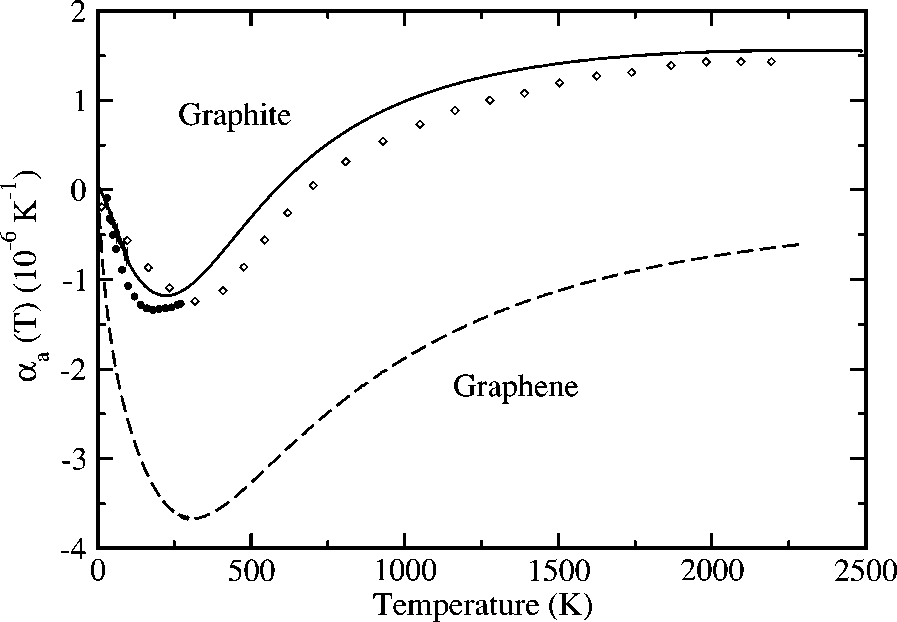
\includegraphics[width=0.8\linewidth]{qha_gra.png}%
\caption{ Thermal expansion coefficients of graphite and graphene calculated using QHA (continuous line) and experimental result for graphite (points). Image source: \cite{Mounet2005} }
\label{fig:qha_gra}
\end{figure}

Equilibrium lattice constants at any temperature $a_0(T)$ are calculated by direct minimization of the Helmholtz free energy $F(a,T)$ with respect to its independent lattice vector, i.e. in this case, $\mathbf{a}$ and $\mathbf{b}$ for black P, and $\mathbf{a}$ for blue P. For the minimization process, $F(a,T)$ is obtained by fitting the discrete data points of $F({a_i,T})$ to the third-order Birch-Murnaghan equation of state, where $i$ is the label for different lattice constants or equivalently different strains. The $F({a_i,T})$ is constructed from $\omega^i_{\mathbf{q},j}$ and $E[a_i]$ through the following formula\cite{QHA0,QHA1}:
\begin{equation}\label{eq:free-enerji}
F({a_i,T}) = E[a_i]+\sum_{\mathbf{q},j}\frac{\hbar \omega^i_{\mathbf{q},j}}{2} +k_BT\sum_{\mathbf{q},j}\text{ln}\left( 1-\text{exp} \left[ -\frac{\hbar \omega^i_{\mathbf{q},j}}{k_BT} \right]\right).
\end{equation}
Here, $T$ is the temperature, $k_B$ is the Boltzmann constant, $E[a_i]$ is the DFT ground state energy. $\omega^i_{\mathbf{q},j}$ is the phonon frequency at the q point $\mathbf{q}$ with band index $j$. 
The sums  run over all q points and all bands of the whole Brillouin zone. Since the structural instabilities arise especially for the armchair direction when under compressive strain values larger than 4\%,  the calculation of phonon dispersions for both structures are performed under small strains, namely $\pm$ 2\%,  in order to evaluate $\omega^i_{\mathbf{q},j}$ and $E[a_i]$. Considering two independent lattice vectors \textbf{a} and \textbf{b} of black P two uniaxial strains are applied for these directions. While for blue P, only biaxial strain is applied to keep its hexagonal symmetry unchanged. The whole calculation process was carried out using phonopy-qha script\cite{phonopy-qha}.

\subsubsection{Computational details}

\begin{footnotesize}
\begin{description}
\item[Simulation program:] VASP and Phonopy\cite{phonopy_code}
\item[Energy cut-off:] 500 eV
\item[Pseudopotentials:] PBE-GGA(PAW)
\item[k points (Monkhorst-Pack):] 15$\times$11$\times$1 and 15$\times$15$\times$1 for black P and blue P, respectively 
\item[Vacuum:] 25~\AA
\item[Energy and force convergence criterion:] 10$^{-5}$ eV and 10$^{-7}$ eV/\AA, respectively
\item[Supercell for phonon calculation:] 7$\times$3$\times$1 and 5$\times$5$\times$1 for black P and blue P, respectively
\item[q points for phonon calculation:] 200$\times$200$\times$1
\end{description}
\end{footnotesize}

\subsection{Phonon modes and dispersion \label{sec:pho_phos}}

Different from a pure planar graphene, black P and blue P have a buckled non-planar structure due to the sp$^3$ hybridization, yet all three structures share the same hexagonal lattice base. Given an almost identical local environment in the unit cell, see \autoref{fig:phos_struc}, it is not surprising that blue P and black P having similar total energy. Only significant difference is the plane, marked as grey shown in \autoref{fig:phos_struc}, on which the system extends to form an infinite 2D crystal. Therefore, thermal expansion on these different planes are expected to be different and will carry insight information on the different finite temperature properties. The primitive unit cell of black P is a rectangular lattice with a four-atom basis and a space group of $D_{2h}^7$, and that of blue P is a hexagonal lattice with a two-atom basis and a space group of  $D_{3d}^3$. Therefore, besides the three acoustic modes with the in-phase vibrations of atoms, there are nine and three optical modes for black P and blue P, respectively. 

\begin{figure}[htbp]
\centering
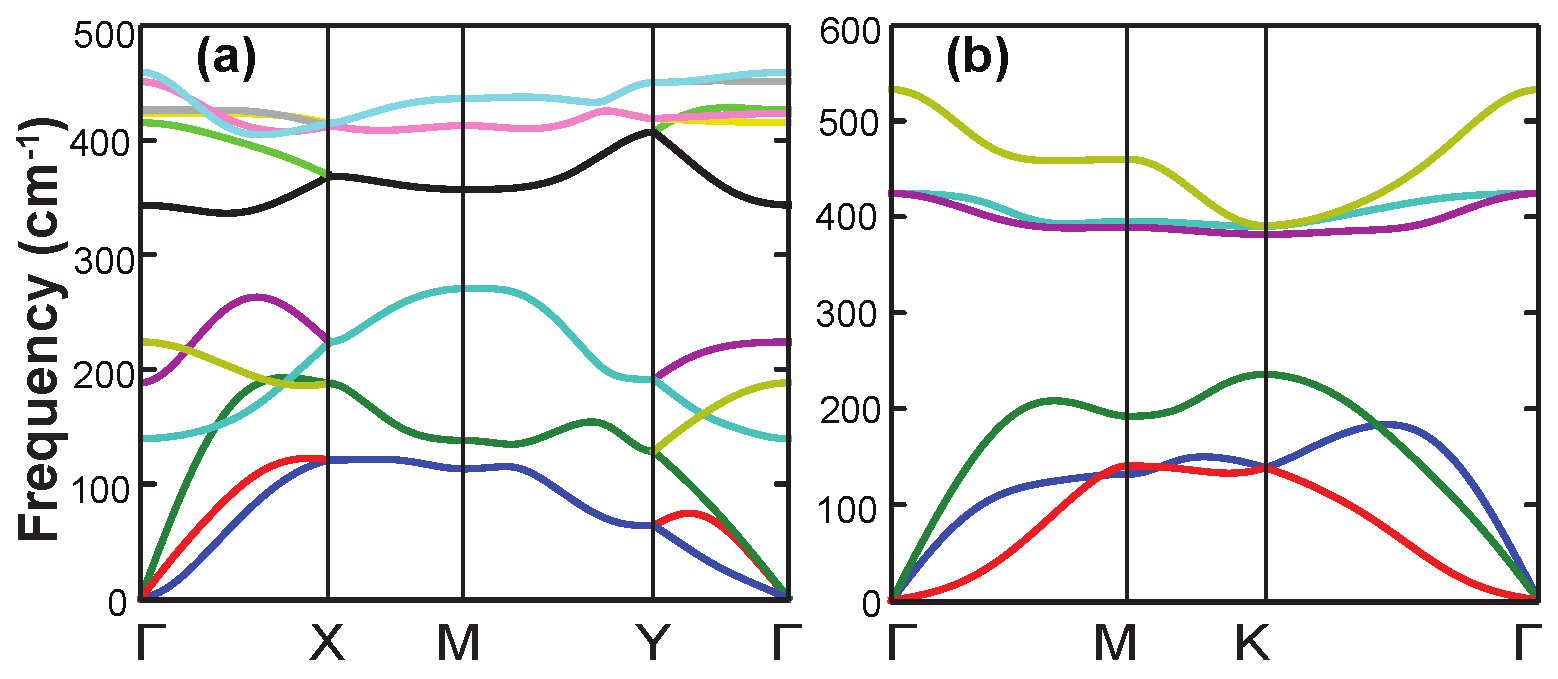
\includegraphics[width=0.8\linewidth]{phos_phon.eps}%
\caption{Calculated phonon dispersions for prinstine (a) black and (b) blue P. (c) Optical phonon modes together with their frequencies (in units of cm$^{-1}$) at the $\Gamma$ point and irreducible representations for black P and blue P.\label{phos_phon}}
\end{figure}

The calculated phonon dispersions along the high symmetric q lines corresponding to these modes are depicted in \autoref{phos_phon}(a) and (b) for both structures. Parallel with the previous calculations~\cite{phonon-blackP,phonon-blackP-1}, the calculated phonon dispersions are free from imaginary frequencies, which ensures the structural stability of the materials. Lowest acoustic mode ZA displays a $q^2$ relation as we discussed in \autoref{chap:3}.  The other two acoustic modes LA and TA still have a linear dependence with respect to the $q$ wavevector since the situation is the same here as in the bulk. The total frequency range of the phonon dispersion is larger by an amount of about 100 cm$^{-1}$ in blue P as compared to black P. We will discuss more about the vibrational character of these phonon modes in the later chapters where we investigate the effect of strain on the frequency of the vibration.

\subsection{Results of temperature-dependent thermal properties}

The equilibrium lattice constants at zero K, $a_0$ and $b_0$ of black P and $a_0$ of blue P, are predicted as $a_0$ = 3.298 {\AA}, $b_0$=4.625 {\AA}, and  $a_0$ = 3.277 {\AA}, respectively,  in  good agreement with previously reported results ($a_0$ = 3.297 {\AA}, $b_0$=4.640 {\AA} for black P\cite{fei,dcakir}, and  $a_0$ = 3.330 {\AA} for blue P\cite{Zhu2014}). 
The expansion of these lattice parameters due to zero-point vibration is around 0.2\% at 0 K, which is smaller than that of other well-known two dimensional materials like graphene and $h$-BN, but it is comparable with that of MoS$_2$ and MoSe$_2$. This result is reasonable due to the difference in the maximum phonon frequency between these materials: that of graphene and $h$-BN is around 1600 cm$^{-1}$ and that of MoS$_2$, MoSe$_2$, black P and $a_0$ of blue P is around 600 cm$^{-1}$. 

\begin{figure}[htbp]
\centering
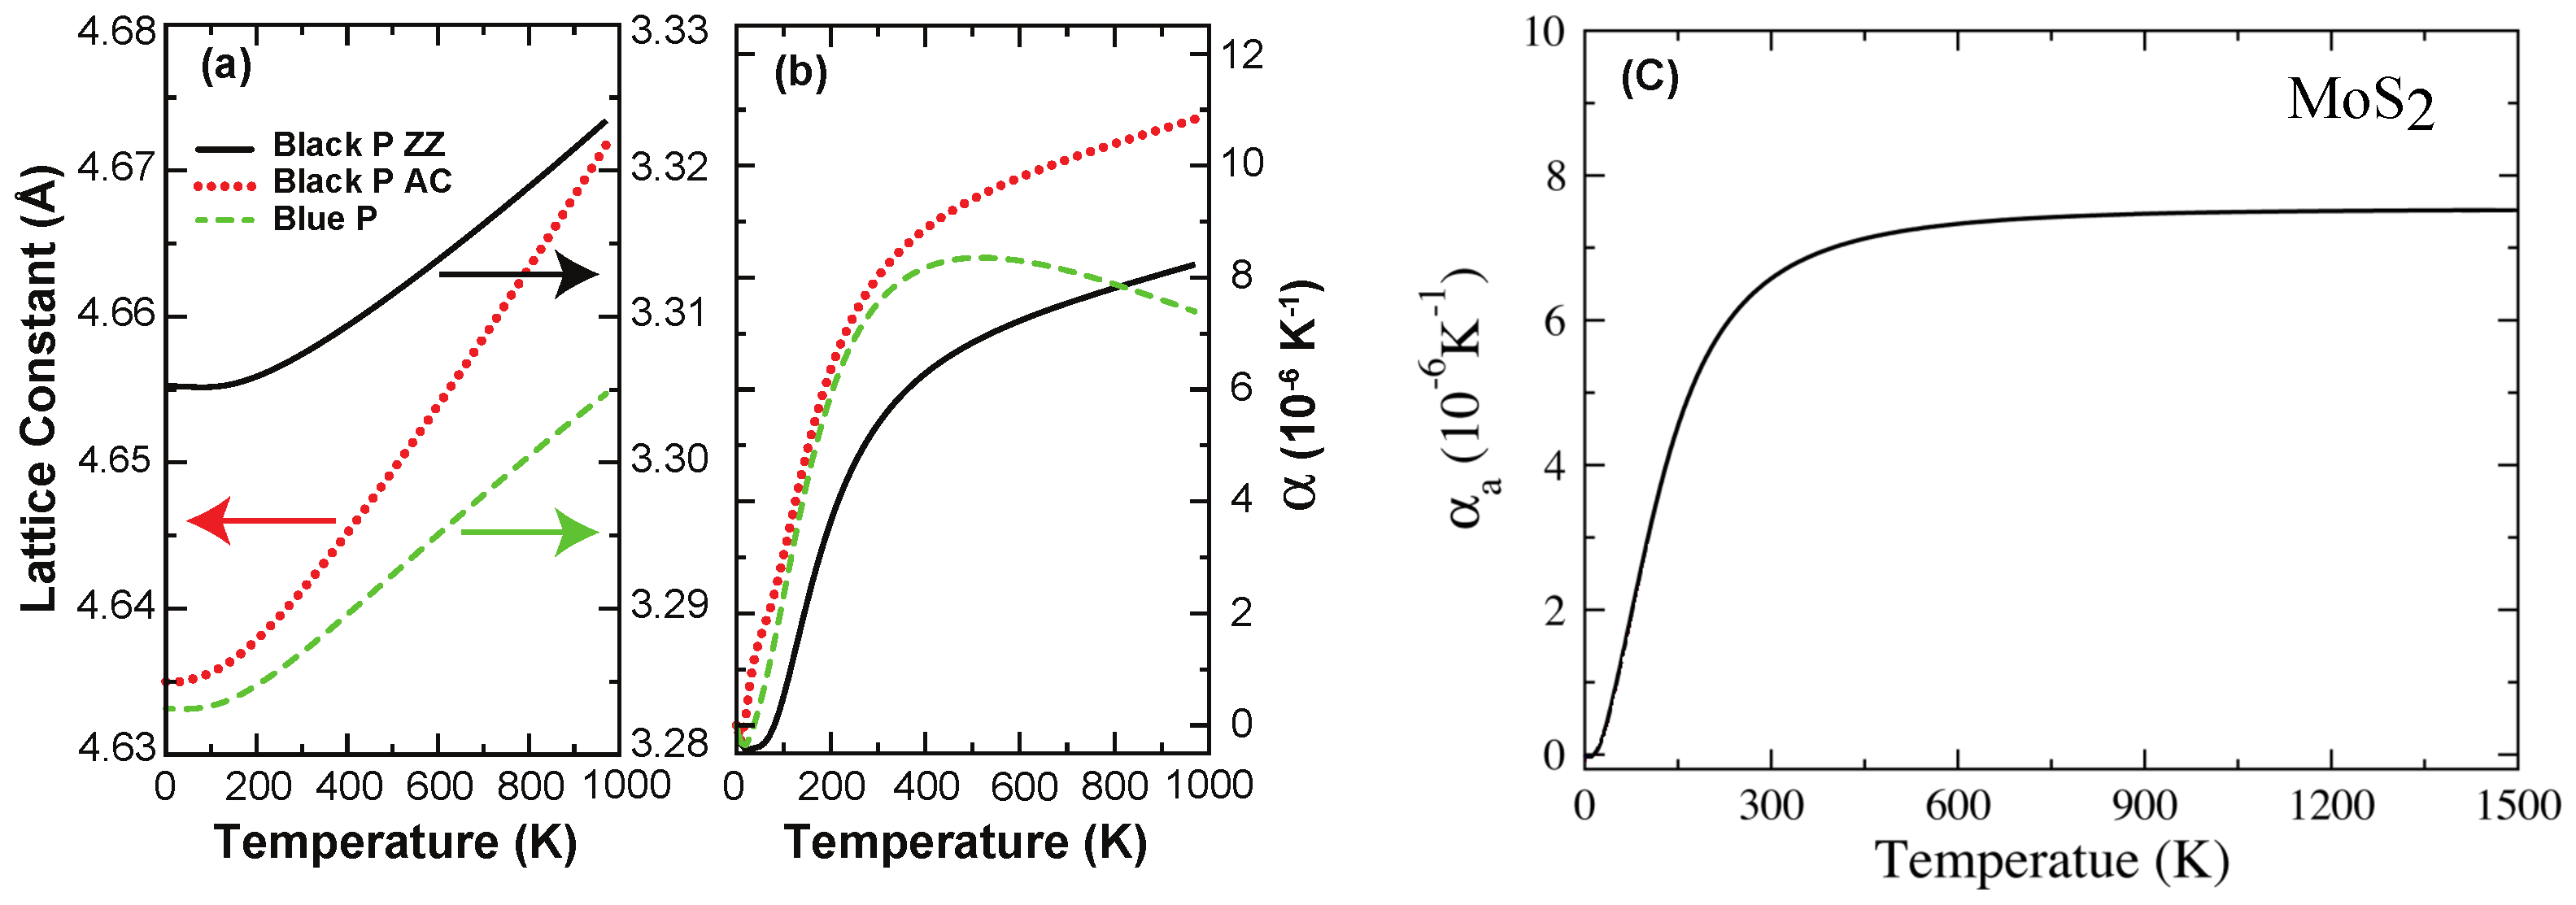
\includegraphics[width=\linewidth]{expan_T.eps}%
\caption{(a) Lattice constants and (b) TEC as a function of temperature.  Here, ZZ and AC are denoted for the zigzag and armchair directions, respectively. (c) TEC of monolayer MoS$_2$ for comparison from Ref. \cite{QHA3}.\label{fig:tec}}
\end{figure}

The temperature dependence of the lattice constants $a_0(T)$, $b_0(T)$ and thermal expansion coefficients (TEC) $\alpha(T)$ of both structures are shown in \autoref{fig:tec}. Anisotropic nature of the structure of black P leads to different lattice constant expansion rates. A faster thermal expansion along the armchair direction (i.e. $\mathbf{b}$) is found, see \autoref{fig:tec}(a). While a small negative TEC appears for all structures in all directions at temperatures lower than 100 K, black P along the zigzag direction has a more apparent negative expansion.  The lattice constant of both phases varies linearly when T $>$ 200 K, see \autoref{fig:tec}(a). The TEC increases rapidly with temperature  up to 300 K.  After that, all TECs changes slowly with temperature starting from around 400 K in agreement with predictions for two-dimensional transition metal dichalcogenides~\cite{QHA2,QHA3}, for example see \autoref{fig:tec}(c) for monolayer MoS$_2$.
Different from MoS$_2$, we do not observe any saturation of the TEC for black P at high temperatures.  While black P expands at most 0.02 {\AA} along the zigzag direction as T approaches 1000 K, it expands 0.04 {\AA} along the armchair direction. As is clear from \autoref{fig:phos_struc}, an uniaxal expansion along the armchair direction may result in a structural phase transition from black P to blue P because of the similar hexagonal arrangement of P atoms\cite{negative-pos}. 

\begin{figure}[htbp]
\centering
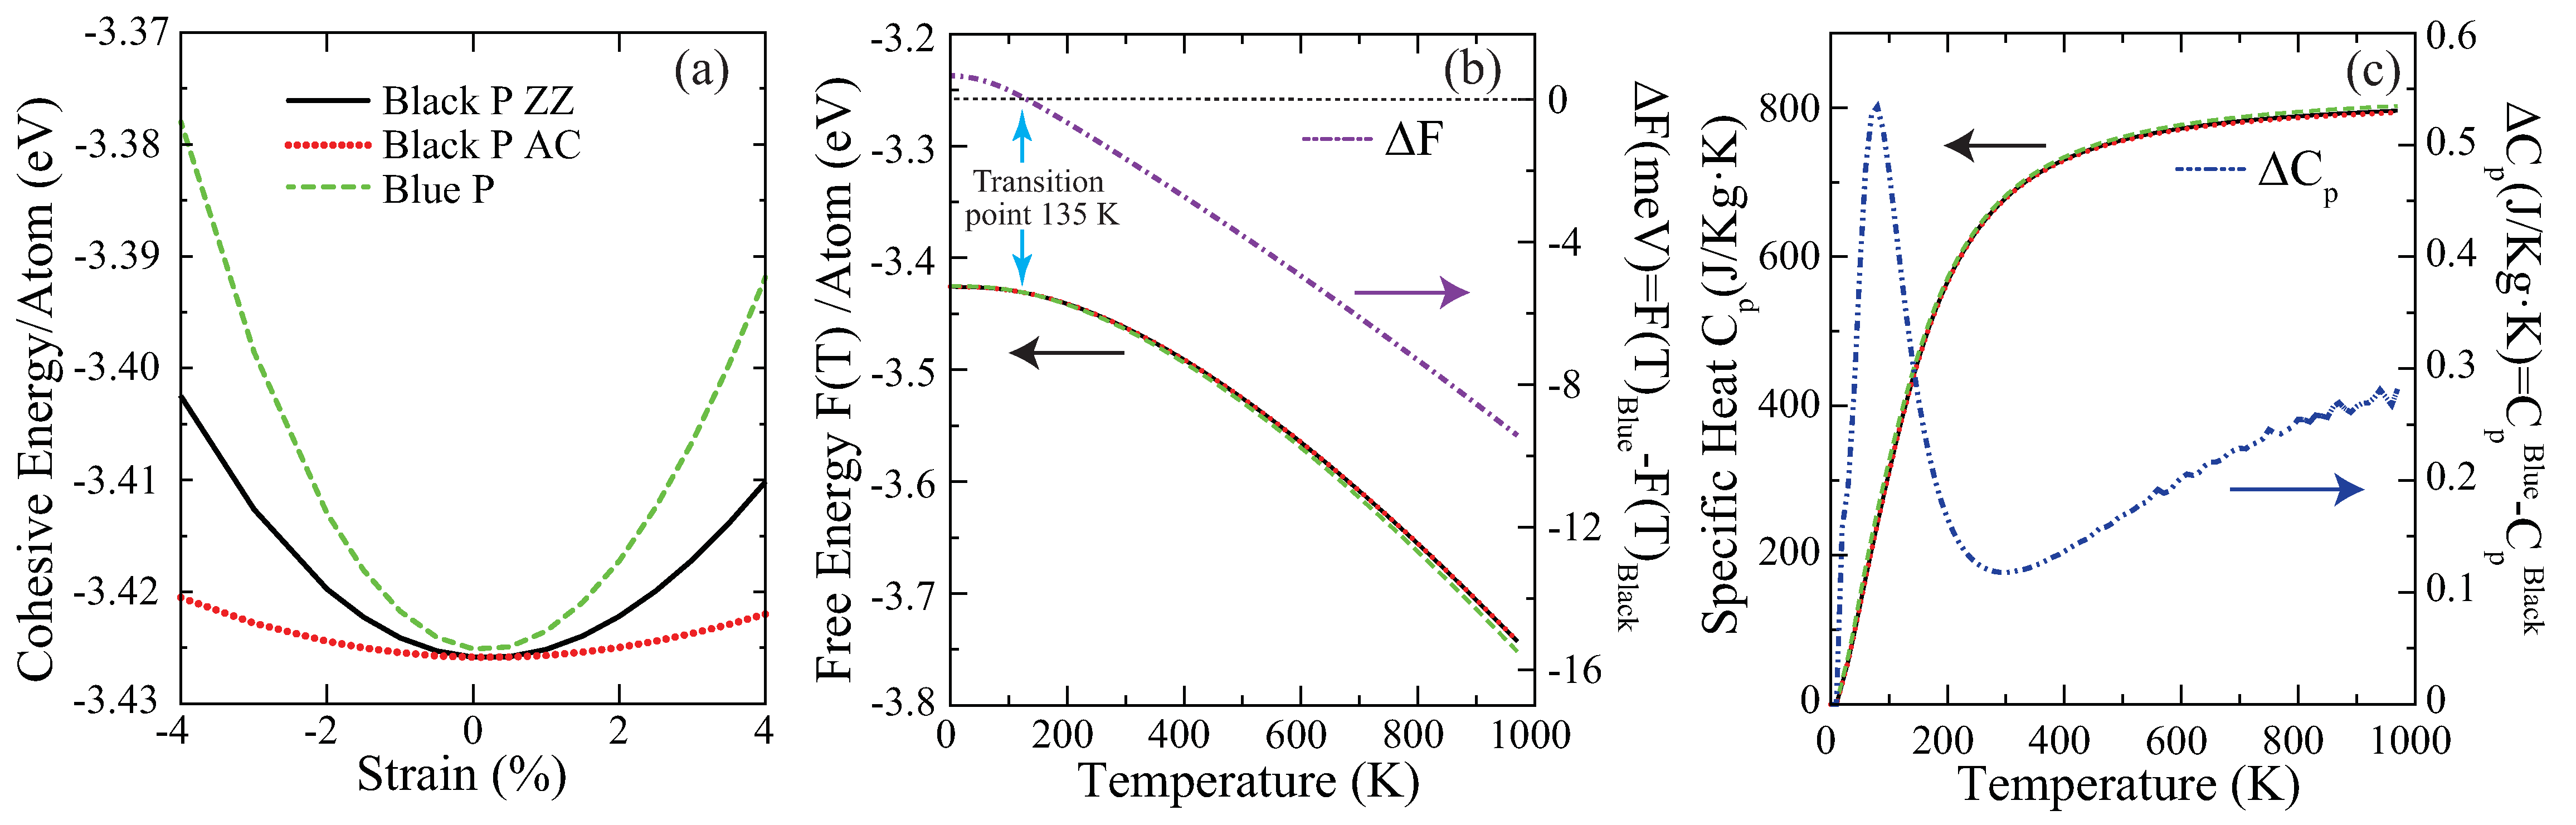
\includegraphics[width=\linewidth]{freeE_T.eps}%
\caption[Thermal properties variations of phosphorene with temperature]{(a) Cohesive energy, including zero point energy, as a function of applied strain at $T$ = 0 K and (b) Helmholtz free energy ($F(T)$) as a function of temperature.  Here, ZZ and AC are used for the zigzag and armchair directions, respectively. $\Delta F(T)$ is the difference between $F(T)$ of black P and blue P. The blue arrow  (b) denotes the transition point, after which blue P becomes thermodynamically more stable over black P.  The specific heat at constant pressure ($C_p$) and the difference ($\Delta C_p$) between $C_p$ of black P and blue P are shown in (c).  \label{energies_data}}
\end{figure}

In \autoref{energies_data}, the variation of the cohesive energy as a function of strain at 0 K (a) and the variation of the Helmholtz free energy (F(T)) as a function of temperature (b) are presented. In \autoref{energies_data}(b), 
we also show $\Delta F(T)$ which is defined as $\Delta F(T)$=$F_{blue P}(T)$ - $F_{black P}(T)$. Here, $F_{blue P}(T)$ and $F_{black P}(T)$ are the Helmholtz free energy of black P and blue P, respectively. As the zero-point energy continuously decreases with strain from minus to plus, the variation of the zero-point energy results in an asymmetric behaviour in cohesive energy with strain. In addition, the curvature of this total energy gives the in-plane stiffness of the material as a measure of the response to mechanical deformation. It is clear that blue P is a stiffer material as compared to black P.  Moreover, the deformation along the zigzag direction of black P is harder than that along the armchair direction at 0 K, and this is consistent with the finite temperature behaviour as we conclude from previous section in connection with \autoref{fig:tec}(a). 

The $F(T)$ decreases as temperature increases due to the entropy term (the last term in \autoref{eq:free-enerji}). Inclusion of the zero-point energy gives rise to a slightly higher ground state energy for blue P over black P since its optical phonon modes have larger frequencies. However, as temperature increases, a crossing of the free energy curves around 135 K occurs, which makes the blue P energetically more favorable at high temperatures, see \autoref{energies_data}(b). The free energy difference between the two phases is of the order of 4 meV at room temperature, meaning that the two phases can coexist. In addition, it is possible to observe a phase transition driven by temperature from black P to blue P or visa verse at T=135 K. 

In \autoref{energies_data}(c), we present constant pressure heat capacity, $C_p$, results for both structures, which is generally few percent differ from constant volume heat capacity in similar structures\cite{QHA1}. The $C_p$ difference ($\Delta C_p$) between two phases is significantly small for all temperature range as represented with blue dash dot line in \autoref{energies_data}(c), which states essentially very similar Debye temperature for these two different phases.  At high temperatures, C$_p$ approaches its classical value of 12 $k_B$.  When T=300 K, C$_p$ already reaches about 80 $\%$ of its classical value, meaning that the most of the phonon modes are activated at this temperature. 

\subsection{Summary}

In summary, we systematically investigate the lattice thermal properties of black and blue P. Similar to its electronic properties, black P has direction dependent mechanical and thermal properties. The calculated thermal expansion coefficients demonstrate that a much larger expansion along the armchair direction with temperature is observed for black P. While black P is thermodynamically more stable than blue P, the latter becomes more stable when T $>$ 135 K, yet their free energy difference is small due to their structural similarities. It is possible to observe a structural phase transition from black P to blue P by increasing temperature beyond 135 K, and therefore the coexistence of these two phases is possible. 

\section[Piezoelectric properties of 2D-TMDCs and 2D-TMDOs]{Piezoelectric properties of 2D-TMDCs and 2D-TMDOs \footcite[This work is published in:][]{Menderes2015}}

We have seen the general properties of 2D-TMDs in \autoref{chap:1} and vibrational and electronic properties of their one member: 2D-MoS$_2$ in \autoref{chap:3}. When the S atom is replaced with O, TMDs become transition metal dioxides (TMDOs), whose monolayer have similar properties as 2D-TMDs. For the consistency with the paper, here in this section we refer to the 2D-TMDs as 2D-TMDCs. Although 2D-TMDOs proven to be stable, they have not been synthesis yet. Sharing similar electronic strucutre, 2D-TMDCs and 2D-TMDOs already demonstrating various of potential applications, such as nanoelectronic and nanophotonic devices for their direct finite band gaps\cite{Jariwala2014,Wang2012}. In addition to these exciting applications, 2D-TMDCs in the noncentrosymmetric 2H crystal structure with $D_{3h}$ symmetry have also been shown to have remarkable piezoelectric properties that can be then use in pressure sensors,  transducers,  high voltage generators,  nonlinear energy harvesters, energy conversion and piezotronic applications. Many layered materials have a centrosymmetry which suppresses the piezoelectricity. However, this symmetry will be broken when it searches the monolayer level, and then the piezoelectricity is recovered. For example, graphene preserves the centrosymmetry as in graphite, or inversion symmetry, due to its non-polar nature thus it does not display piezoelectricity; Whereas 2D-BN and 2D-TMDs break such symmetry and become noncentrosymmetric system where piezoelectric effect can manifest themselves. 

\citet{Duerloo2012} calculated the piezoelectric properties of single layer of BN, MoS$_2$, MoSe$_2$, MoTe$_2$, WS$_2$, WSe$_2$, and WTe$_2$by using first principle calculations. They reported that piezoelectricity of the 2D-TMDC monolayers in H phase are comparable or even better than that of conventional bulk piezoelectric materials. \citet{Zhu2014a} reported 
experimental evidence of piezoelectricity in free-standing MoS 2 and they found that this material exhibits piezoelectricity for an odd number of layers in which case inversion symmetry is broken. Their measured piezoelectric coefficient is 2.9$\times$10$^{-10}$ C/m, which agrees well with previous theoretical calculations\cite{Duerloo2012}.  Similarly, by using DFT based theoretical calculations, it has been predicted that group III monodichalcogenides, namely GaS, GaSe and InSe, have piezoelectric stress coefficients of 1.34$\times$10$^{-10}$, 1.34$\times$10$^{-10}$ and 1.47$\times$10$^{-10}$ C/m, respectively\cite{Li2015}.  In addition, reducing the dimensionality has been shown to enhance piezoelectricity in ZnO\cite{Xiang2006}. These studies indicate that TMDCs are promising candidates as low dimensional piezoelectric materials. 

Since previous calculations and experiments were only focused on Mo and W based TMDs, the potential of other 2D-TMDCs and 2D-TMDOs for piezoelectric device applications have remained an open question so far. To reveal such potential, first principles calculations are performed in order to systematically investigate the piezoelectric properties of single layer 2H-MX$_2$ compounds, where M= Cr,  Mo, W, Ti, Zr, Hf, Sn and X=O, S, Se, Te.  Lattice parameters, atomic positions, electronic band-gap values, elastic stiffness constants ($C_{11}$ and $C_{12}$), Young modulus ($Y$), Poisson's ratios ($\nu$), piezoelectric stress coefficients ($e_{11}$) and piezoelectric strain coefficients ($d_{11}$) are calculated. 

\subsection{Piezoelectric constants}

Piezoelectricity is the ability of some materials to generate internal electric field in response to applied mechanical stress. Two types of piezoelectric phenomenons can be observed for piezoelectric materials: 1) direct piezoelectric effect: separation of opposite charge due to stress and 2) converse piezoelectric effect: occurrences of stress and strain under external electric field. In \autoref{fig:piezo}, the mechanism of direct piezoelectric effect is shown. 

\begin{figure}[htbp]
\centering
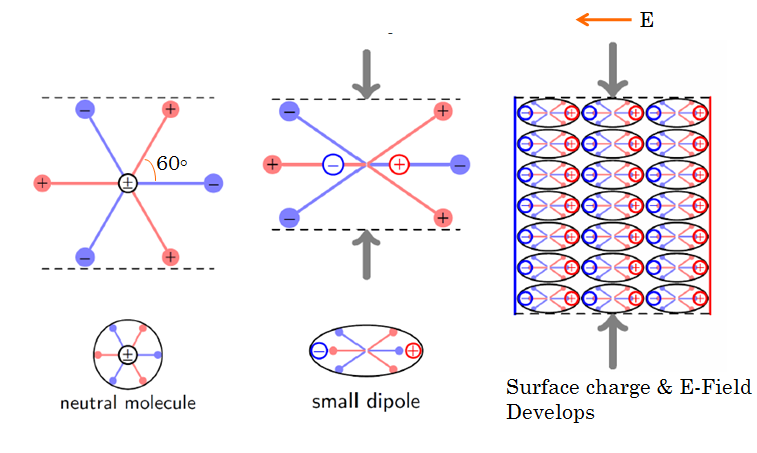
\includegraphics[width=0.8\linewidth]{piezo.png}%
\caption{Mechanism of direct piezoelectric effect\label{fig:piezo}. Image source: \cite{piezo_fig}}
\end{figure}

To investigate the piezoelectric properties, we follow the same theoretical approach of Ref. \cite{Duerloo2012}. The piezoelectric tensor\cite{RevModPhys.73.515,PhysRevB.72.035105}, $e_{ij}$, can be defined  in terms of the induced polarization in the  direction $i$ due to a strain ($\varepsilon_{j}$) change along the direction $j$ as follows
\begin{equation}
e_{ij}=\partial P_{i}/\partial\varepsilon_{j}=\partial P_{i}/\partial\varepsilon_{j}\mid_u+\sum_k (\partial P_{i}/\partial u_{ik})(\partial u_{ik}/\partial\varepsilon_{j}). \label{eq:equ1}
\end{equation}
where $P_i$ is the induced polarization along the direction $i$ as a result of an applied strain $\varepsilon_{j}$ along the direction $j$. 
The $P_i$ is calculated using the Berry Phase approach\cite{vanderbilt2000} as implemented in the VASP package with applied uniform strain, ranging from 0.01 \% to -0.01 \% in steps of 0.005 \%, along the armchair side of the rectangular cell. At this point, in order to apply strain in a desired direction, the hexagonal primitive cell structure of each material is transformed to a tetragonal one composed of two hexagonal primitive cells\cite{Duerloo2012}, see \autoref{fig:mx2_str}. The first term in \autoref{eq:equ1} is the clamped-ion or homogeneous strain contribution to the piezoelectric tensor and it mainly arises from the electronic contribution. The second term represents the contribution from the internal relaxation of ions. Here, $u_{ik}$ is the fractional coordinate of the $k^{th}$ atom along the $i$ direction of the unit cell. 

Since TMDCs and TMDOs compounds have a non-centrosymmetric crystal structure, the inclusion of internal relaxation becomes essential in order to obtain realistic piezoelectric properties. In addition, it is clear that the relaxed-ion piezoelectric coefficients are experimentally relevant quantities that can be measured. From the theoretical point of view, since the relaxed-ion piezoelectric coefficients include both electronic and relaxation effects, the calculation of the clamped-ion piezoelectric coefficients helps to separate the electronic and relaxation contributions from the relaxed-ion piezoelectric coefficients. The number of independent piezoelectric tensor coefficient is deduced from the symmetry of the crystal. For TMDCs and TMDOs, we only need to calculate the $e_{11}$ component of the piezoelectric stress tensor. $e_{11}$ relates in-plane strain to in-plane electrical polarization. The piezoelectric coefficient $e_{31}$ is zero due to the presence of an inversion centre between the two layers of chalcogenides. However, it is found to be non-zero for the unsymmetrical H and F co-decorated graphene\cite{Ong2013,KIM201462}. 

The corresponding piezoelectric strain tensor ($d_{11}$) of each material is predicted from the following relation\cite{Duerloo2012}:
\begin{equation}\label{eq:d11}
                d_{11}= e_{11}/( C_{11} - C_{12} ).
\end{equation}
For each applied strain, the ions are kept in their strained positions or allowed to relax to their new equilibrium positions, and consequently the clamped-ion or relaxed-ion piezoelectric properties are calculated, respectively.

\begin{figure}[htbp]
\centering
	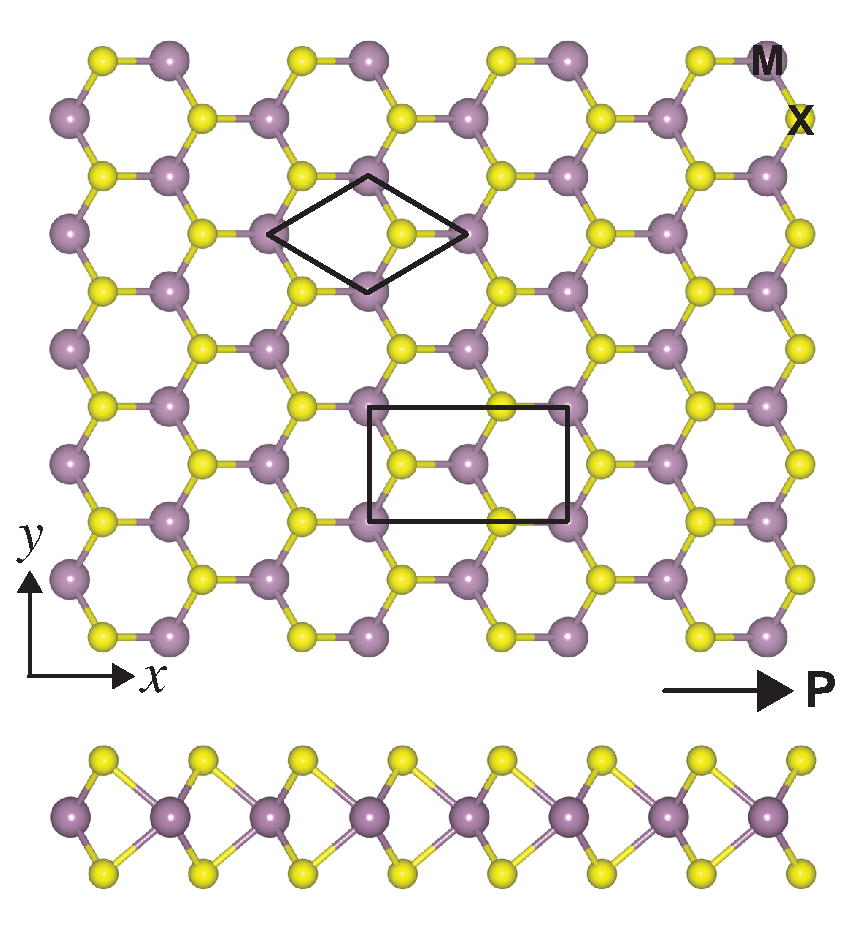
\includegraphics[width=0.5\linewidth]{mx2_str.eps}
	\caption{Top and side views of MX$_2$ where M= Cr,  Mo, W, Ti, Zr, Hf, Sn and X=O, S, Se, Te. P denotes the direction of the polarization. Piezoelectric calculations are done in a rectangular cell. \label{fig:mx2_str}}
\end{figure}

\subsubsection{Computational details}

\begin{footnotesize}
\begin{description}
\item[Simulation program:] VASP
\item[Energy cut-off:] 600 eV
\item[Pseudopotentials:] PBE-GGA(PAW), HSE06
\item[k points (Monkhorst-Pack):] 26$\times$26$\times$1
\item[Vacuum:] 15~\AA
\item[Energy and force convergence criterion:] 10$^{-3}$ eV and 10$^{-7}$ eV/\AA, respectively
\item[strain applied:] 1\% to -1\% in steps of 0.5\%
\item[stress and force:] finite displacement method
\item[polarization:] Berry Phase expression \cite{vanderbilt2000} in VASP
\end{description}
\end{footnotesize}

\subsection{Accurate band gaps from HSE06 hybrid functional}

It is mandatory that a piezoelectric material has to be an insulator or semiconductor with a sufficiently wide band gap to avoid current leakage. Thus, we first calculate the electronic properties of twenty eight single layer MX$_2$ compounds, where M= Cr,  Mo, W, Ti, Zr, Hf, Sn and X=O, S, Se, Te. We discard the metallic structures, namely SnSe$_2$, SnTe$_2$, and TiTe$_2$. Actually, G$_0$W$_0$ calculations predicted that 2H-TiTe$_2$ is a small band gap semiconductor material\cite{Rasmussen2015}. Since semi-local functionals are used in the Berry's phase calculations, 2H-TiTe$_2$ is excluded. For electronic structure calculations, we also applied the HSE06 hybrid functionals in order to obtain realistic electronic band gap values for TMDCs and TMDOs. \autoref{fig:bandgaps} shows the calculated PBE-GGA and HSE06 band gap values E$_{gap}$. The materials, except Cr, Mo, and W based TMDCs, have indirect band gaps and the predicted values and trends are in good agreement with previous theoretical calculations\cite{Duerloo2012,Ataca2012,Guo2014}. Generally, the band gap increases when moving upwards in the chalcogens family from Te to S and with increasing atomic number in the transition metals. However, the latter trend is partially valid when the compounds with O are included. The difference is that within the same row of the transition metals, TMDOs with a larger atomic number tend to have smaller band gaps which is in contrast to the TMDCs case.

\begin{figure}[htbp]
\centering
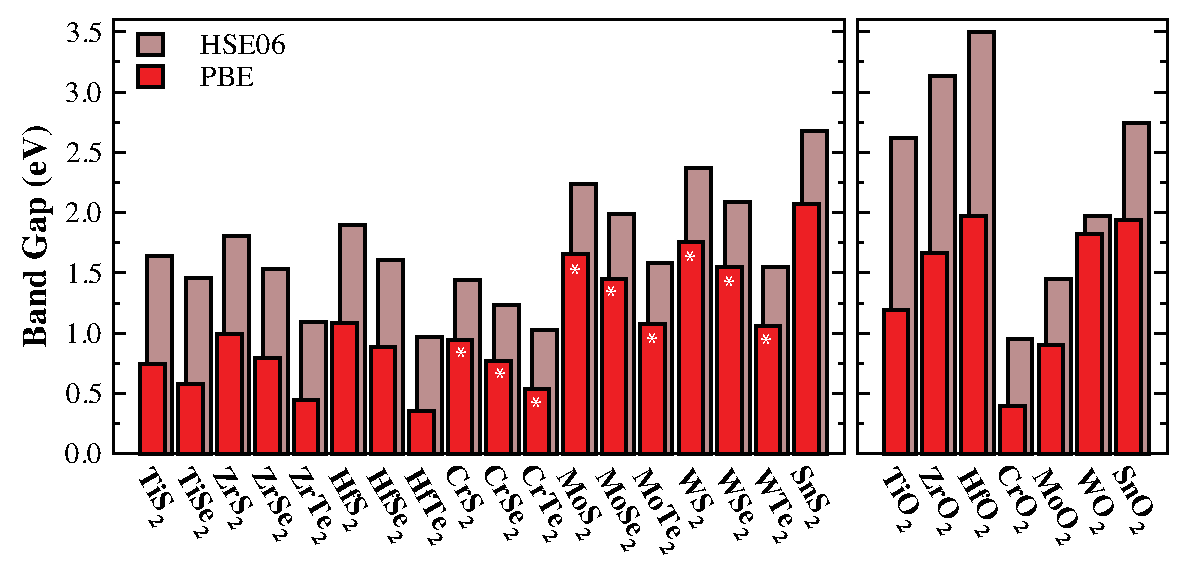
\includegraphics[width=0.8\linewidth]{bandgaps.eps}
\caption{\label{fig:bandgaps}The calculated PBE-GGA and HSE06 E$_{gap}$ values for TMDCs and TMDOs. Here, white * sign indicates that it is a direct band gap material.}
\end{figure}

\subsection{Elastic constants}\label{elastic}

\begin{table}[htbp]
\centering
\caption{\label{tab:elastic}Calculated clamped and relaxed-ion elastic constants (in units of N/m), Young modulus Y (in units of N/m) and Poisson's ratio $\nu$.  }
\begin{tabularx}{\linewidth}{lXXXXsXXXX}
 \hline\hline
 Material& \multicolumn{4}{c}{Clamped Ion} && \multicolumn{4}{c}{Relaxed Ion}\\\cline{2-5}\cline{7-10}
 &  $C_{11}$ & $C_{12}$ & $Y$ & $\nu$ && $C_{11}$ & $C_{12}$ & $Y$ & $\nu$ \\\hline
TiS$_2$ & 100.3 &  34.2 &  88.6 & 0.34 &&  89.9 & 28.6 &  80.8 & 0.32\\
TiSe$_2$ & 84.8 &  29.3 &  74.7 & 0.35 &&  74.4 & 24.4 &  66.4 & 0.33\\
ZrS$_2$ &  96.3 &  37.7 &  81.5 & 0.39 &&  84.2 & 31.8 &  72.2 & 0.38\\
ZrSe$_2$ &  83.3 &  31.0 &  71.8 & 0.37 &&  71.4 & 26.0 &  61.9 & 0.36\\
ZrTe$_2$ &  66.2 &  22.8 &  58.35 & 0.34 &&  53.1 & 18.6 &  46.6 & 0.35\\
HfS$_2$ & 104.4 &  39.1 &  89.8 & 0.37 &&  92.8 & 33.8 &  80.5 & 0.36\\
HfSe$_2$&  89.7 &  32.2 &  78.1 & 0.36 &&  78.8 & 27.8 &  69.0 & 0.35 \\
HfTe$_2$&  71.0 &  23.5 &  63.2 & 0.33 &&  59.3 & 19.7 &  52.8 & 0.33 \\
CrS$_2$ & 136.9 &  42.6 & 123.6 & 0.31 && 120.6 & 32.3 & 111.9 & 0.27\\
CrSe$_2$& 111.3 &  37.5 &  98.7 & 0.34 &&  96.6 & 28.9 &  87.9 & 0.30\\
CrTe$_2$&  86.5 &  32.7 &  74.1 & 0.38 &&  73.0 & 25.8 &  63.9 & 0.30\\
MoS$_2$ & 157.2 &  50.1 & 141.2 & 0.32 && 132.7 & 33.0 & 124.5 & 0.25\\
MoSe$_2$& 133.2 &  40.8 & 120.7 & 0.31 && 106.9 & 25.6 & 100.8 & 0.24\\
MoTe$_2$& 106.3 &  32.8 &  96.2 & 0.31 &&  84.1 & 19.8 &  79.4 & 0.24\\
WS$_2$  & 174.7 &  51.9 & 159.3 & 0.30 && 146.5 & 31.8 & 139.6 & 0.22\\
WSe$_2$ & 147.4 &  41.1 & 135.9 & 0.28 && 102.4 & 23.1 & 115.9 & 0.23\\
WTe$_2$ & 115.4 &  31.6 & 106.8 & 0.27 &&  89.2 & 15.7 &  86.4 & 0.18\\
SnS$_2$ &  92.8 &  23.1 &  87.1 & 0.25 &&  91.0 & 22.2 &  85.6 & 0.24\\
TiO$_2$ & 178.9 &  80.9 & 142.3 & 0.45 && 173.7 & 75.7 & 141.7 & 0.44\\
ZrO$_2$ & 163.5 &  83.0 & 121.5 & 0.51 && 157.4 & 77.5 & 119.2 & 0.49\\
HfO$_2$ & 181.7 &  86.7 & 140.3 & 0.48 && 174.2 & 81.5 & 136.1 & 0.47\\
CrO$_2$ & 233.8 &  87.4 & 201.1 & 0.37 && 218.6 & 74.4 & 193.3 & 0.34\\
MoO$_2$ & 253.3 & 104.0 & 210.6 & 0.41 && 230.2 & 84.5 & 199.2 & 0.37\\
WO$_2$  & 286.2 & 109.0 & 244.7 & 0.38 && 261.2 & 87.8 & 231.7 & 0.34\\
SnO$_2$ & 165.7 &  52.4 & 149.1 & 0.32 && 160.2 & 53.3 & 142.5 & 0.33\\
\hline\hline
\end{tabularx}
\end{table}

As previously mentioned, we need to calculate the elastic constants in order to obtain the piezoelectric strain, $d_{11}$ coefficients, see \autoref{eq:d11}. Therefore, the relaxed-ion and clamped-ion elastic stiffness coefficients (C$_{11}$ and C$_{12}$), Young modulus (Y= (C$_{11}^2$-C$_{12}^2$)/C$_{11}$) and Poisson's ratios ($\nu$=C$_{12}$/C$_{11}$ ) for all 2D-TMDC and 2D-TMDO materials considered in this study are obtained and are listed in \autoref{tab:elastic}. Our results are in good agreement with available data\cite{Peng2013,Kang2013,Duerloo2012,Cooper2013}. The first observation from \autoref{tab:elastic} is that C$_{11}$, C$_{12}$ and Y decreases with increase of the row number of the chalcogenide atom. Except Zr, in each chalcogenide group, the MX$_2$ monolayer becomes stiffer with increase of the row number of the metal atom. Structures considered in this study are found to be less stiff when compared to graphene (Y=341 N/m)\cite{cakir2014} and single layer $h$-BN (Y=275.9 N/m)\cite{cakir2014}. Also it should be noticed that the calculated elastic constants are positive and satisfy the Born stability criteria for crystals having hexagonal symmetry\cite{Nye1957,Born1998}.  Note that the relaxed-ion elastic constants, i.e. C$_{11}$ and C$_{12}$, are always smaller than the clamped-ion ones since the internal relaxation of ions allows to release some of the stress in the former, see \autoref{tab:elastic}.

\subsection{Piezoelectric stress/strain coefficients}\label{piezo}

\begin{figure}[htbp]
\centering
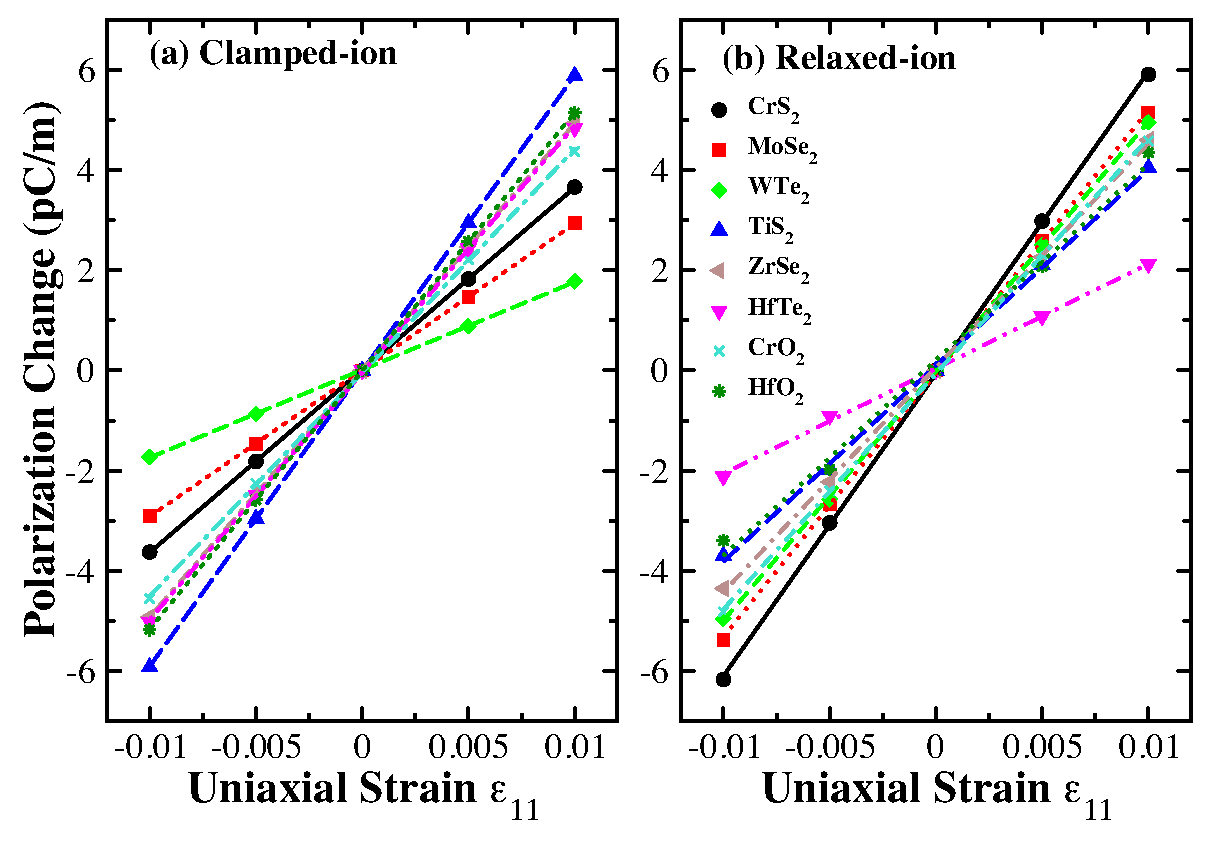
\includegraphics[width=0.8\linewidth]{polariz.eps}
\caption{\label{fig:polariz} (a) Clamped-ion and (b) relaxed-ion polarization change under applied uniaxial strain ($\varepsilon_{11}$) along the $x$ direction for the selected 2D-TMDCs and 2D-TMDOs structures. Piezoelectric coefficient is determined from the slope of the curves.}
\end{figure}

\begin{figure}[t]
\centering
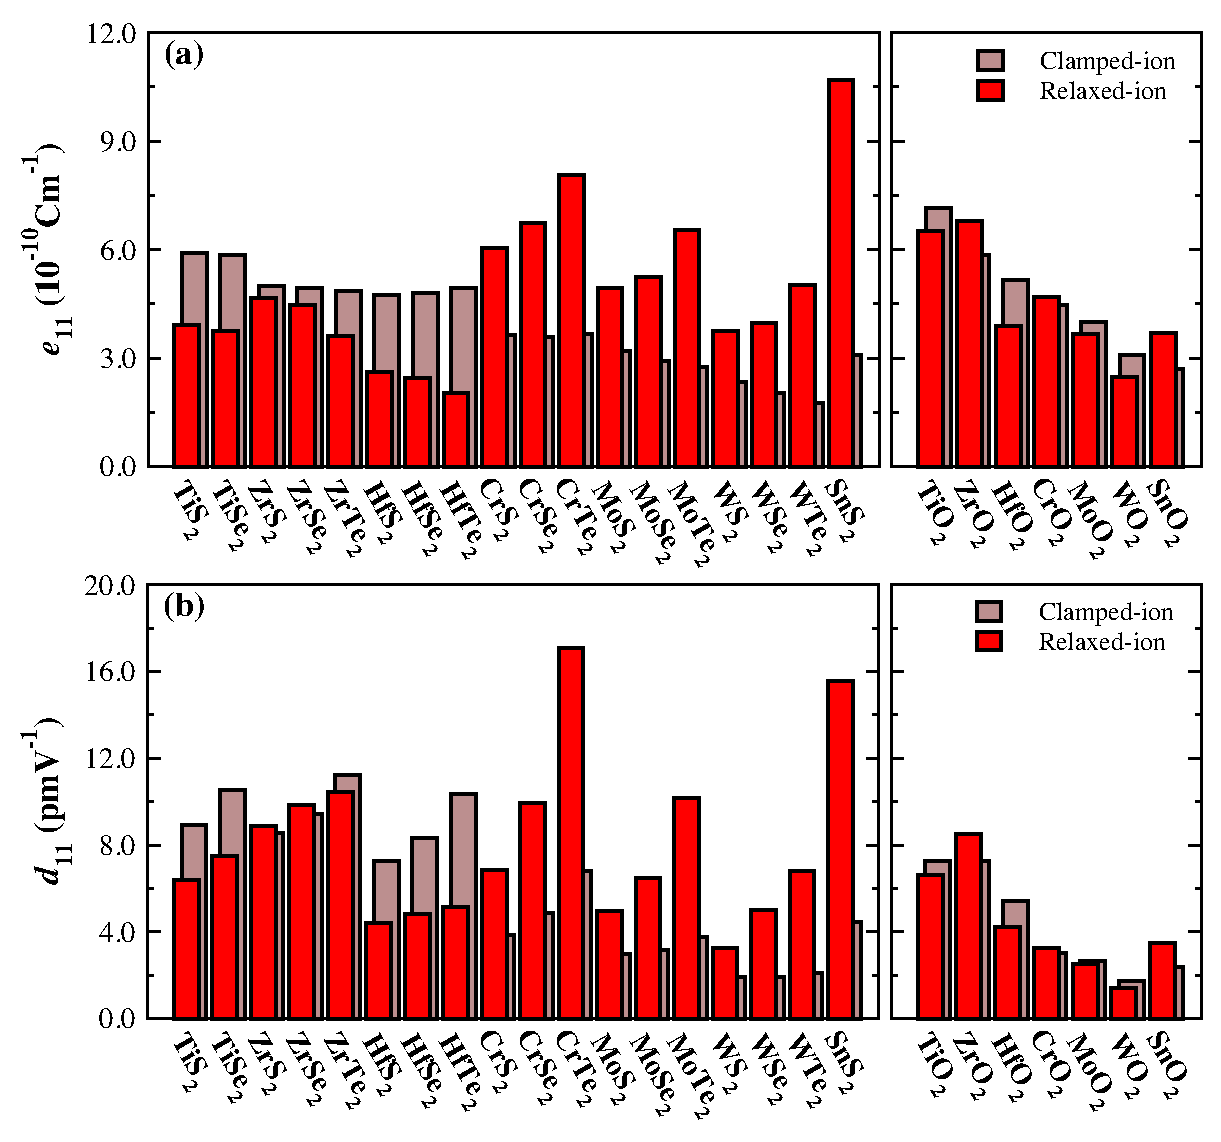
\includegraphics[width=0.8\linewidth]{piezo_res.eps}
\caption{\label{fig:piezo_res}The calculated clamped and relaxed-ion (a) piezoelectric stress ($e_{11}$)  and (b) piezoelectric strain ($d_{11}$) coefficients.}
\end{figure}

Piezoelectric coefficients ($e_{11}$) are derived from the slope of the polarization change in \autoref{fig:polariz}) with applied uniform strain, ranging from 0.01 \% to -0.01 \% in steps of 0.005 \%, along the armchair side of the rectangular cell via Berry's Phase approximation\cite{vanderbilt2000}. The clamped-ion and relaxed-ion $d_{11}$ coefficients are obtained by using the calculated $e_{11}$ coefficients, and the elastic constants ($C_{11}$ and $C_{12}$) via \autoref{eq:d11}. \autoref{fig:piezo_res} shows the calculated $e_{11}$ and $d_{11}$ coefficients for both TMDCs and TMDOs. The materials are ordered along the $x$-axis by considering the period and group number of the transition metal element in the periodic table. The predicted relaxed-ion $e_{11}$ and $d_{11}$ coefficients are consistent with the available reference data\cite{Duerloo2012,crs2}, see results for Cr, Mo and W based TMDCs, which are comparable with the piezoelectric properties of single layer and bulk $h$-BN\cite{Duerloo2012,km-2009,km-2011a,km-2011b}. In addition, the relaxed-ion $e_{11}$ coefficient of single layer MoS$_{2}$ (4.91$\times$10$^{-10}$ C/m) is comparable with the experimentally measured piezoelectric coefficient of 2.90$\times$10$^{-10}$ C/m\cite{Zhu2015} and agrees  well  with the reported value of 3.64$\times$10$^{-10}$ C/m.\cite{Duerloo2012}. In addition, the trends found for the $e_{11}$ and $d_{11}$ coefficients of Mo and W based TMDCs are consistent with those found in Ref.\cite{Duerloo2012}. The difference between our calculated piezoelectric coefficients and previous calculations is likely due to the use of different pseudopotentials, small differences in elastic constants, and other computational parameters (for instance $k$-mesh).

SnS$_2$ has the highest $e_{11}$ coefficient for the relaxed-ion (10.7$\times$10$^{-10}$ C/m) calculation. WO$_2$ has the smallest relaxed-ion piezoelectric stress coefficient (2.49$\times$10$^{-10}$ C/m) among TMDOs and WTe$_2$ has the smallest clamped-ion piezoelectric stress coefficient (1.75$\times$10$^{-10}$ C/m). From \autoref{fig:piezo_res}, we predict several  periodic trends in clamped-ion $e_{11}$ and $d_{11}$ coefficients for TMDC and TMDO monolayers. The clamped-ion $e_{11}$ coefficients of TMDCs usually increase when moving from right to left in the periodic table (i.e., from CrX$_{2}$ to TiX$_{2}$) and upward in an individual group of both transition metal and chalcogen atoms.  This trend is nearly the same for TMDOs. However, for TMDCs, the trend (i.e., the increase in the calculated clamped-ion $e_{11}$ coefficients when moving upward in the group of chalcogen elements) becomes reversed for the relaxed-ion calculations of group VI elements  as clearly seen in \autoref{fig:piezo_res}(a). 
The clamped and relaxed ion $d_{11}$ coefficients increase when moving downward in the group of chalcogen elements (i.e. from S to Te) in each metal group.  This trend can be correlated to the polarizability of chalcogen atoms since the atoms are easily polarized when going downward in a specific group of the periodic table.  We notice that the chalcogenide atoms have a much larger impact on the $d_{11}$ coefficients as compared to the metal atoms.  Especially in group VI, the $d_{11}$ coefficient is maximized if one uses a smaller metal atom and a larger chalcogen atom. In group IV, Zr does not exhibit the same trend that is found for the group VI elements. This is partially because the C$_{11}$ elastic constant of Zr based TMDCs for a particular chalcogen atom is smaller that that of Ti and Hf based TMDCs. Since TMDOs pose larger elastic constants, they usually have smaller $d_{11}$ coefficients as compared to TMDCs. In other words, the stronger the material the smaller the $d_{11}$ coefficient.  

Among the group VI elements (i.e., Cr, Mo and W), Cr based TMDCs and TMDOs are found to have much better piezoelectric properties in each chalcogenide group and CrTe$_2$ possesses the largest relaxed-ion  $e_{11}$ (8.06$\times$10$^{-10}$ C/m) and $d_{11}$ (17.1 pm/V) coefficients. On the other hand, the relaxed-ion $e_{11}$ and $d_{11}$ coefficients of SnS$_{2}$ are  almost the same as those of CrTe$_2$. The predicted relaxed-ion $e_{11}$ values are much larger than the values previously predicted for surface decorated graphene structures\cite{Ong2012}. Furthermore, when the piezoelectric coefficients of the extensively used bulk piezoelectric materials, namely 2.3 pm/V for  $\alpha$-quartz\cite{Bechmann1958}, 3.1 pm/V for wurtzite GaN\cite{Lueng2000} and 5.1 pm/V for AlN\cite{Lueng2000}, are considered, we predict that TMDCs and TMDOs have comparable or even larger relaxed-ion piezoelectric coefficients.

\subsection{Importance of internal relaxation}

It is  essential to discuss the effect of the internal relaxation on the piezoelectric properties of TMDCs and TMDOs. Relaxing the ion positions after applying strain significantly reduces (increases) the polarization of the  Ti, Zr and Hf (Cr, Mo and W) based TMDCs. As a result, the clamped-ion piezoelectric coefficients of the Ti, Zr and Hf (Cr, Mo and W) based TMDCs monolayers are much larger (smaller) than that of the relaxed-ion coefficients. This means that the electronic contribution, i.e. the first term in \autoref{eq:equ1}, and strain contribution, i.e. the second term in \autoref{eq:equ1}, have opposite (the same) sign for the  Ti, Zr and Hf (Cr, Mo and W) based TMDCs.  The calculated elastic constants suggest that Ti, Zr and Hf based TMDCs are more brittle materials that are expected to exhibit larger response to an applied strain, thereby giving rise to higher clamped-ion piezoelectric constants.  For TMDOs, the contribution of internal relaxation to the $e_{11}$ coefficient decrease when moving downward in an individual metal group. 
However, in each chalcogen group, the internal relaxation becomes  generally less important when going from Te to S. This can be attributed to the large strain-induced ionic motion in response of an applied strain. 
In other words, after applying strain, the amount of the internal relaxation of the chalcogen atoms increases from S to Te, giving rise to a larger internal relaxation contribution to the piezoelectric coefficients in Te based TMDCs. 
Since Te is the most easily polarizable atom among the chalcogenide atoms (due to its larger size), the polarization effects (and hence electronic contribution to the  $e_{11}$ coefficient) are found to be large in Te based TMDCs  as compared to S and Se counterparts. However, the increase in piezoelectricity effects competes with the degradation of stability.

\subsection{Summary}

In summary, we presented a detailed theoretical investigation of the piezoelectric properties of semiconductor TMDC and TMDO monolayers. Our calculations show that TMDC and TMDO structures are strong candidates for future atomically thin piezoelectric applications.  We show that Ti,  Zr, Sn and Cr based TMDCs and TMDOs have much better piezoelectric properties as compared to Mo and W based 
TMDCs and TMDOs and the well-known conventional bulk piezoelectric materials.
The usage of these 2D piezoelectric materials in ultra sensitive sensors, low-power electronics and nanoscale electromechanical systems are expected to have an impact on the size reduction, weight and energy consumption of such devices. 

\section[Carrier transport properties of monolayer Titanium trisulfide]{Carrier transport properties of monolayer Titanium trisulfide \footcite[This work is published in:][]{Aierken2016.mobility}}
\subsection{Carrier mobility}
\subsection{Deformation potential theory: non-polar materials}
\subsection{Deformation potential theory: polar materials}

\section[Magnetic properties of penta-hexa-graphene]{Magnetic properties of penta-hexa-graphene \footcite[This work is published in:][]{Aierken2016.magnetism}}
\subsection{Magnetic ordering}
\subsubsection{Stoner criterion of ferromagnetism}

\section[Battery related properties of MXenes/graphene heterostructure]{Battery related properties of MXenes/graphene heterostructure \footcite[This work will be published as:][]{Aierken2017.battery}}
\subsection{Principle of Lithium battery}
\subsection{Key quantities and their modelling}